%!TEX root = ../dynamics.tex
\section{Analyzing the Features Affecting Batch Throughput}\label{sec:throughput}
Now we turn our attention to analyzing the factors that influence the fast progress (or completion) of a batch, how they change, interplay, and their scope overtime.\\

In order to conduct this analysis, we define the task of batch throughput prediction as a machine learning problem with 29 features, some of these features were studied in the previous section while we describe the remaining ones in appendix. The target feature $DIFF\_HIT$ is the numbers of hits that the a given batch would have completed within the next time frame of 1 hour.\\

In practice, to predict the throughput of a batches at time $T$, we a train a Random Forest Regression model with samples taken in the range $[T-\delta, T)$ where $\delta$ is a time window that we are willing to consider for predicting the next outcome. In this process we computed the score\footnote{The used score is the coefficient $R^2$ \cite{sklearn}.} and the mean average error (MAE).
In this experiment we considered the data from June-October 2014 and hourly observations (see section \ref{tracker}), from which we uniformly sampled 50 time points. Finally, for each time point we considered a training time frame $\delta$ ranging from 1hour to 24hours. \\

In figure \ref{fig:accuracy} we see the the computed score reaches its highest values when using the latest 4 hours as a training set, then decreasing when we increase the time frame, to finally again increasing and stabilizing when we used up to 24 hours last hours.\\

\begin{figure}[htbp]
	\centering
		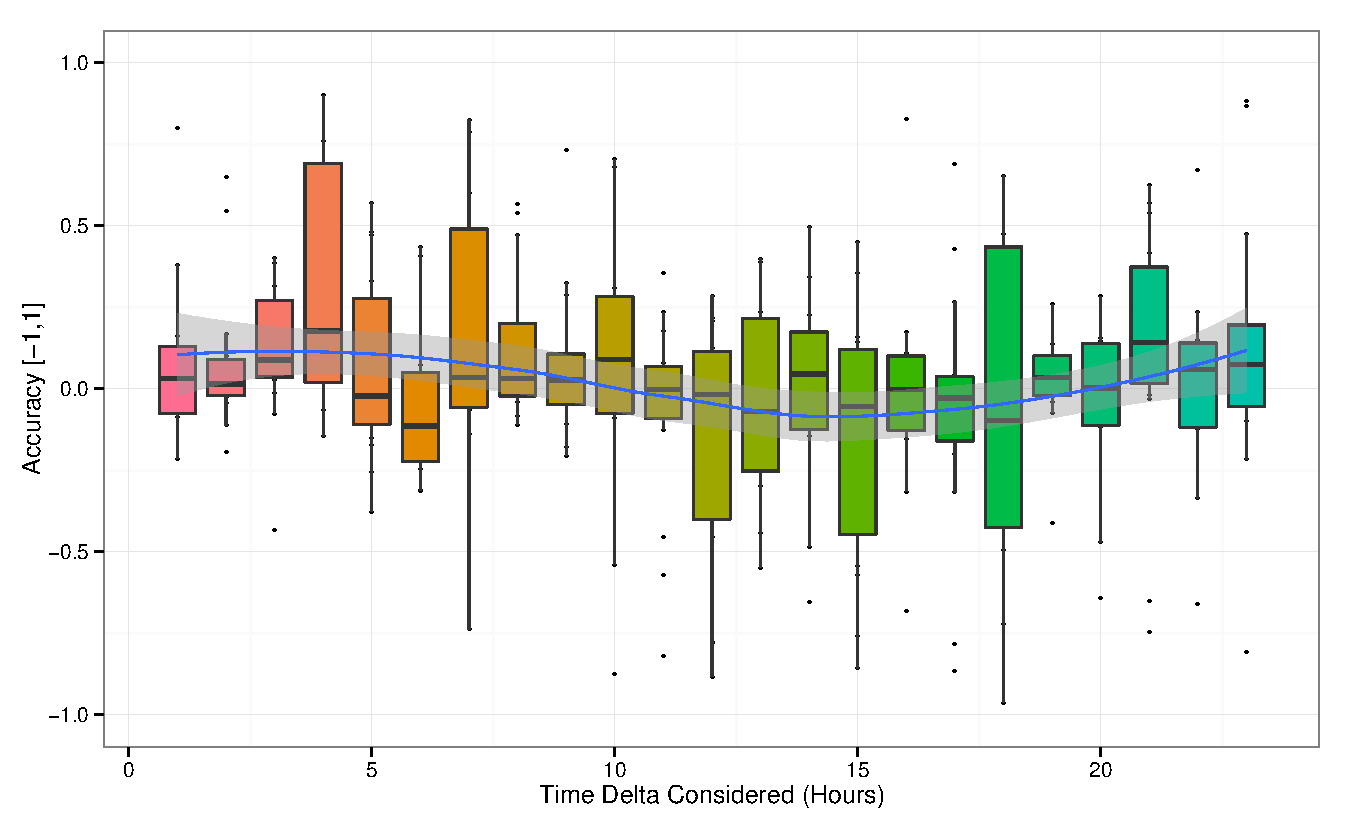
\includegraphics[width=0.5\textwidth]{figures/ML_accuracy}
	\caption{Accuracy of the throughput prediction when considering larger training sets for the prediction.}
	\label{fig:accuracy}
\end{figure}

In order to understand these changes in our prediction we have to look at the features importances that we computed for each training that we run. Figure \ref{fig:importances} shows the percent contribution of each feature and how it varied along when we increased the time frame.
The strongest feature is: $HIT\_Available$, indeed and as observed by many reports, larger batches tend to attract more people, this feature becomes less important when we consider longer periods, partly because of the noise, but most importantly because other features like $Start\_time$ and $left\_minutes$ start encoding additional facts, that is: the crowd is sensible the newly posted hits, or how fresh the hits are.

\begin{figure}[htbp]
	\centering
		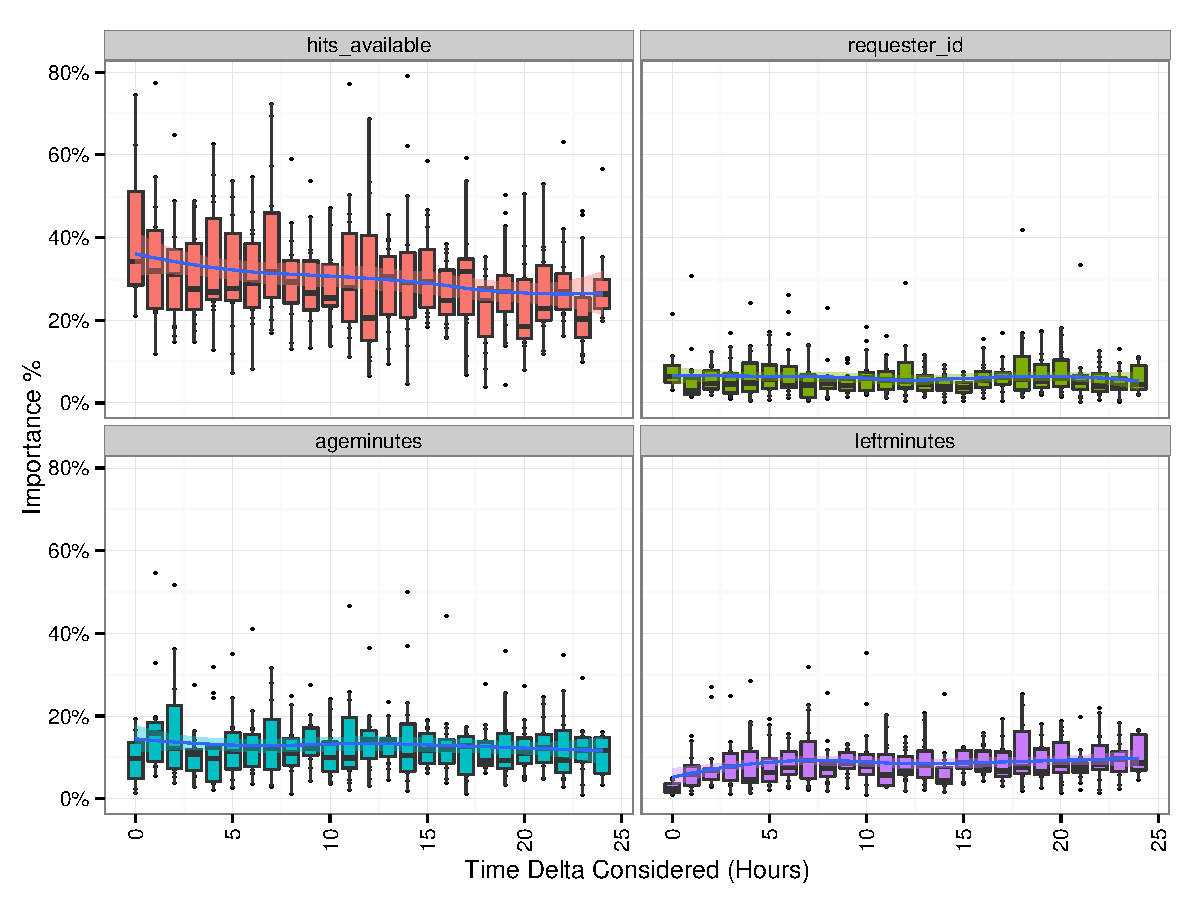
\includegraphics[width=0.5\textwidth]{figures/importances}
	\caption{Feature importance when considering larger training sets for the prediction.}
	\label{fig:importances}
\end{figure}
